\section{System Delimitation}

\subsection{System Environment (statics)}
\subsubsection{System Overview}
The primary purpose of the URL-Archiver is to extract URLs from Unicode text files and PDFs, and archive them on supported platforms: Archive Today and the Wayback Machine. The system provides the archived URL versions to the user via a CSV file. Additionally, when a BibTeX file is provided by the user, the original BibTeX file is updated with a note field containing these archived URLs for each entry.

\subsubsection{Hardware Specifications}
The URL-Archiver does not impose any special hardware requirements. However, an internet connection \index{internet connection} is essential for the archiving process to function.

\subsubsection{Software Components}
The URL-Archiver is platform-independent \index{platform-independent}, operating on major systems such as Windows (tested on Windows 10, version 22H2  and Windows 11, version 23H2), macOS (tested on macOS Sonoma), and Linux (tested on Ubuntu 20.04.3 LTS). The system has varying browser dependencies based on the operating system: Chrome is required for macOS, Edge for Windows, and Firefox for Ubuntu/Linux (Latest stable versions of the browsers are recommended). Users can change the default Browser in the configuration of the application. Other dependencies are installed with the URL-Archiver and do not require separate installation.

\subsubsection{System Architecture}
The URL-Archiver uses the \gls{MVCPattern}\index{Model-View-Controller (MVC) pattern}, as illustrated in figure \ref{fig:mvc_highlevel}, to enable future enhancements, such as adding a \gls{GUI} interface. The \gls{FactoryPattern}\index{Factory Pattern} is applied where appropriate to simplify the extension of functionalities. For instance, adding extra archiving services \index{Archiving Services} can be easily accomplished by introducing a new archiving service, as shown in figure \ref{fig:factory_pattern_archiving_services}.

\begin{figure}
	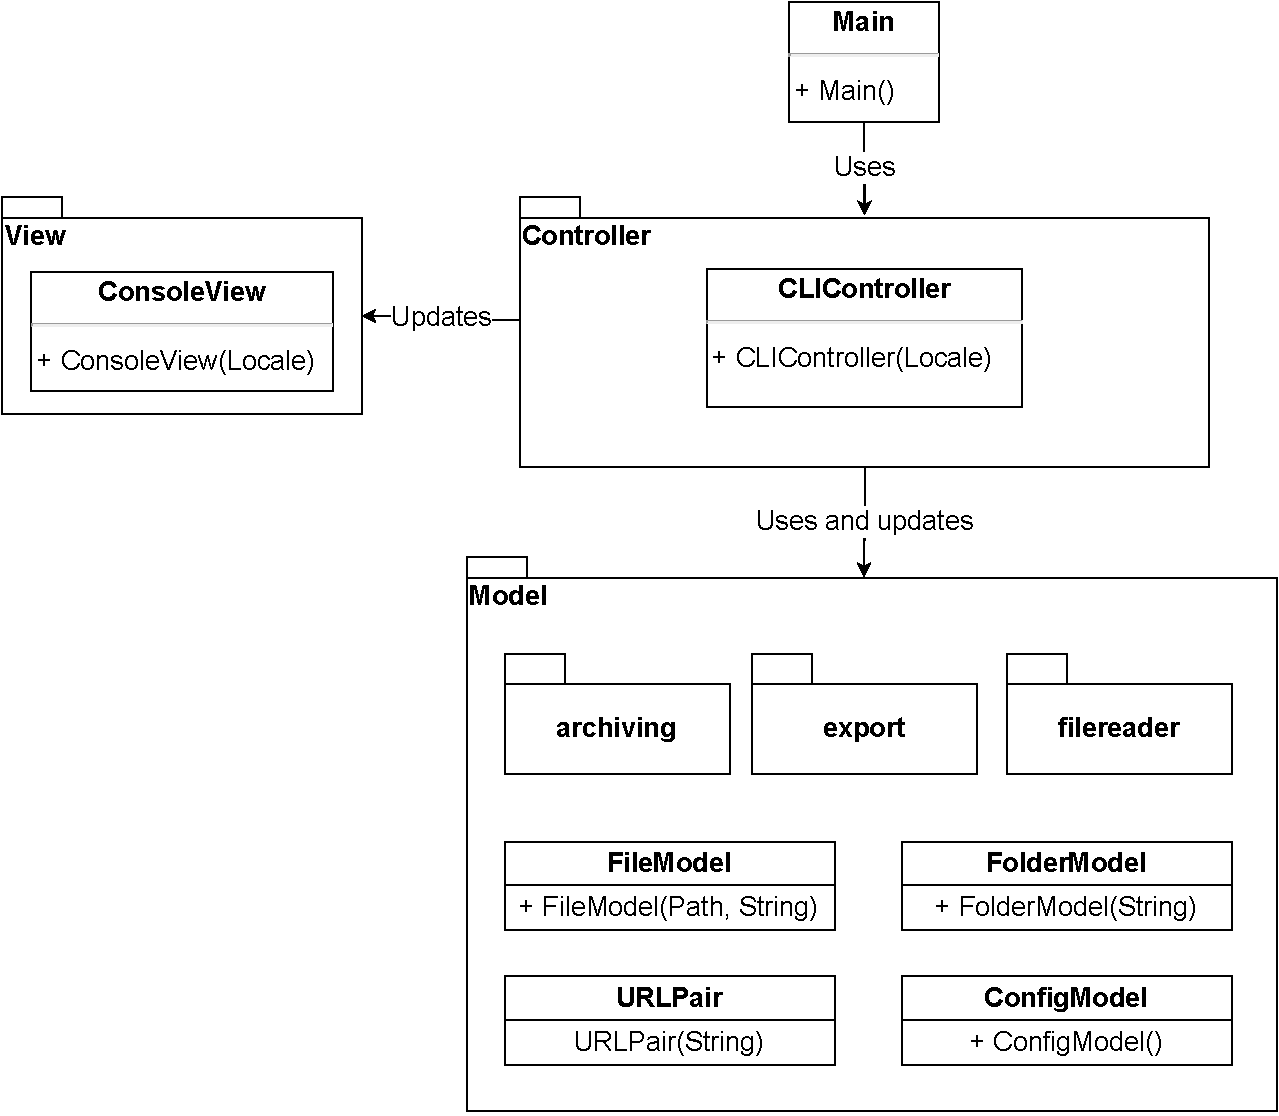
\includegraphics[width=0.5\textwidth]{./diagrams/mvc_diagram-Highlevel_MVC.pdf}
	\centering
	\caption{High-level MVC-Pattern \index{Model-View-Controller (MVC) pattern} from URL-Archiver}
	\label{fig:mvc_highlevel}
\end{figure}

\begin{figure}
	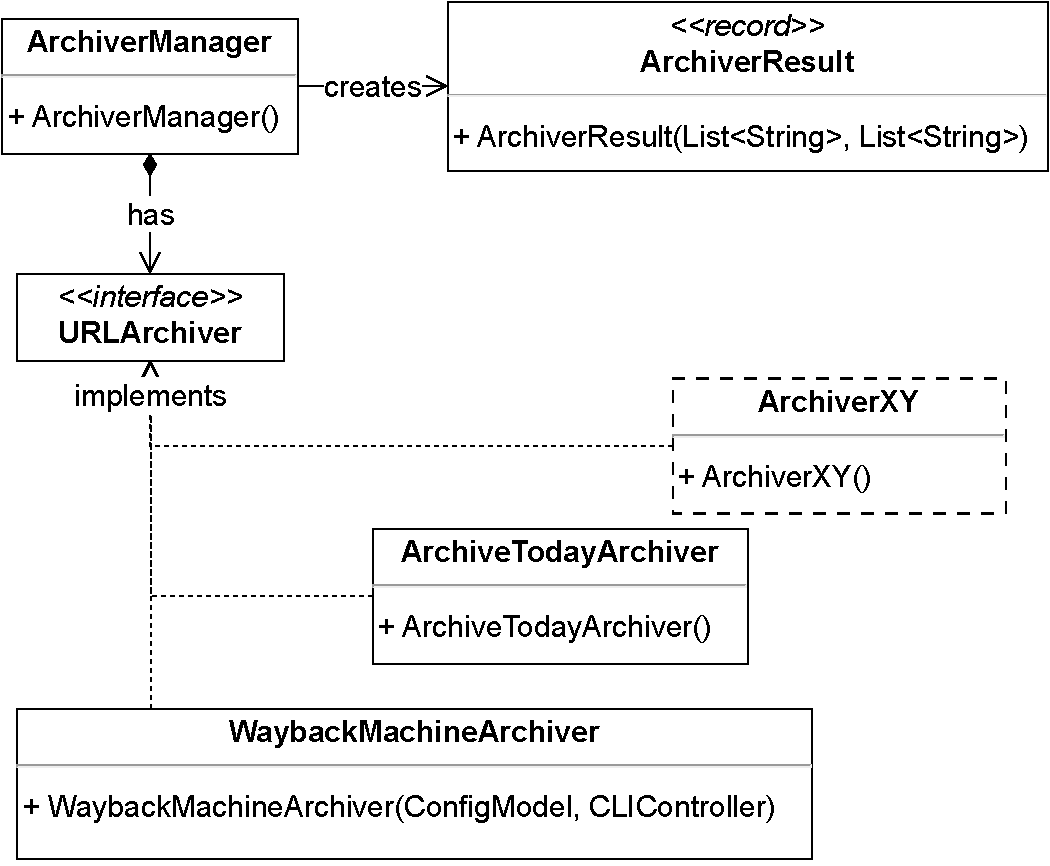
\includegraphics[width=0.5\textwidth]{./diagrams/URL_Archiver_Class_Diagram-ArchiverManager.pdf}
	\centering
	\caption{Extension with new archiving service XY (using the Factory Pattern\index{Factory Pattern})}
	\label{fig:factory_pattern_archiving_services}
\end{figure}

\subsubsection{Data Management}
Upon completion of its execution, the URL-Archiver generates a CSV file where each line contains an extracted URL and its archived versions, separated by semicolons. For example, a line like \texttt{https://xy.com;https://web.archive.org/xy;https://archive.ph/xy} shows the original URL and its archives. This simple format makes it easy to track and manage archived URLs. 

Optionally, if the user provided a BibTeX file, URLs are integrated into the note field of each entry. If there's no existing note field, a new one is created with the format \texttt{note = {Archived Versions: \url{url1}, \url{url2}}}. If a note field already exists, the archived URLs are appended to it in the format \texttt{note = {<current note>, Archived Versions: \url{url1}, \url{url2}}}. This approach ensures that the archived URLs are neatly added to the BibTeX entries, maintaining the integrity of the original data.

\subsubsection{User Interface}
Currently, the system uses a command-line interface. The MVC-Pattern \index{Model-View-Controller (MVC) pattern} lays the groundwork for potential future implementation of a GUI interface.

\subsubsection{Integration with Other Systems}
The system integrates with the Wayback Machine via API, with certain limitations detailed in their API documentation\footnote{https://archive.org/details/spn-2-public-api-page-docs/mode/2up}. For archiving on Archive.today, which lacks an API, Selenium \index{Selenium} is used to automate the process as much as possible. However, users must manually complete captchas.

\subsubsection{Maintenance and Support}
Currently, there are no specified maintenance requirements or a support framework for the URL-Archiver.


\subsection{Process Environment (dynamics)}


\subsubsection{Operational Processes}
The URL-Archiver is initiated by the user, who provides a path to Unicode text or PDF files or a directory that contains such files. The application extracts URLs from these files and presents them sequentially to the user. The user then has options to open or archive that URL. He has also the following other options: 
\begin{itemize}
	\item \textbf{s}: Show a list of previously archived URLs.
	\item \textbf{u}: Update and view pending archive jobs.
	\item \textbf{n}: Navigate to the next URL.
	\item \textbf{q}: Quit the application.
	\item \textbf{c}: Change application settings.
	\item \textbf{h}: Access the Help Menu for assistance.
\end{itemize}

Upon completion, the user is prompted to save URL pairs to a CSV file and, if a Bibtex file is provided, to write the archived URLs back into it. 


\subsubsection{Event Handling}
In the URL Archiver, user actions are efficiently facilitated through the main menu. When archiving a URL, users can select either the Wayback Machine or Archive.today. In addition, the 'c' option in the menu allows users to configure settings, including setting up API keys for the Wayback Machine and selecting a default browser. The application cleverly handles unsupported input and incorrect paths by prompting the user for the correct information or action. This ensures smooth operation and user guidance throughout the process.

\subsubsection{Life Cycle}
The URL-Archiver’s life cycle begins with launch and path input, proceeding to URL extraction and user interactions via the menu options, and ends with prompts for data saving upon completion. See the high-level process in figure \ref{fig:hl_operational_process}.

\begin{figure}[b]
	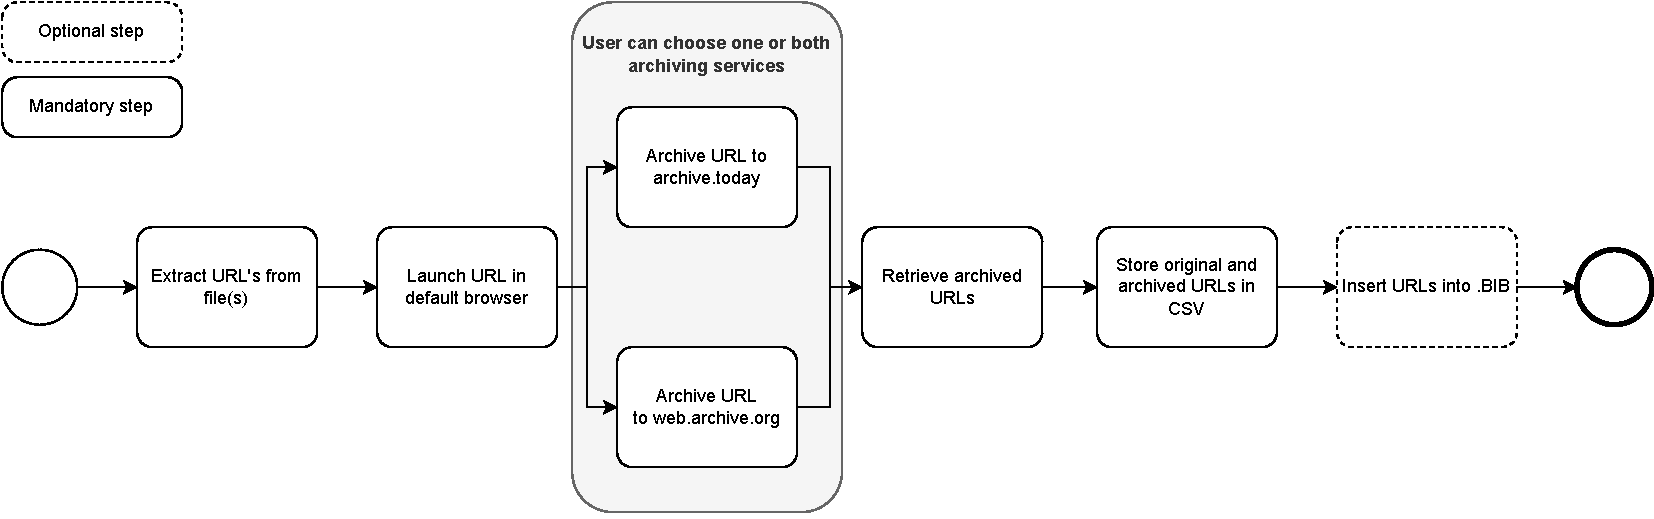
\includegraphics[width=1\textwidth]{./diagrams/process_model-simple-horizontal.pdf}
	\centering
	\index{Archiving Services}
	\caption{High-level operational process}
	\label{fig:hl_operational_process}
\end{figure}

\subsubsection{Error Management}
Errors within the URL-Archiver are caught and handled, typically prompting the user with a customized error message asking to retry the action. No system stack traces are shown to the user.

\subsubsection{Backup and Recovery}
The URL Archiver immediately serialises queued jobs for the Wayback Machine into a JSON file at the start of the archiving sequence. This protocol is designed to preserve the integrity of jobs awaiting execution, thereby increasing the stability of the system in the midst of possible disturbances, including unexpected application terminations. Consequently, it facilitates the recovery of the queue when the application is subsequently activated. It should be noted, however, that URLs that have been successfully archived are not preserved automatically in the current version of the URL Archiver. This feature is a task for future enhancement of the application.

\subsubsection{Update and Upgrade Policies}
Software updates require manual download and recompilation from the Git repository. The system does not provide automatic updates or an in-built feature for update checks.